\newpage
\section{Katarzyna Ludwa}
This is a fox (see Figure~\ref{fig:fox}).
\begin{figure}[htbp]
    \centering
    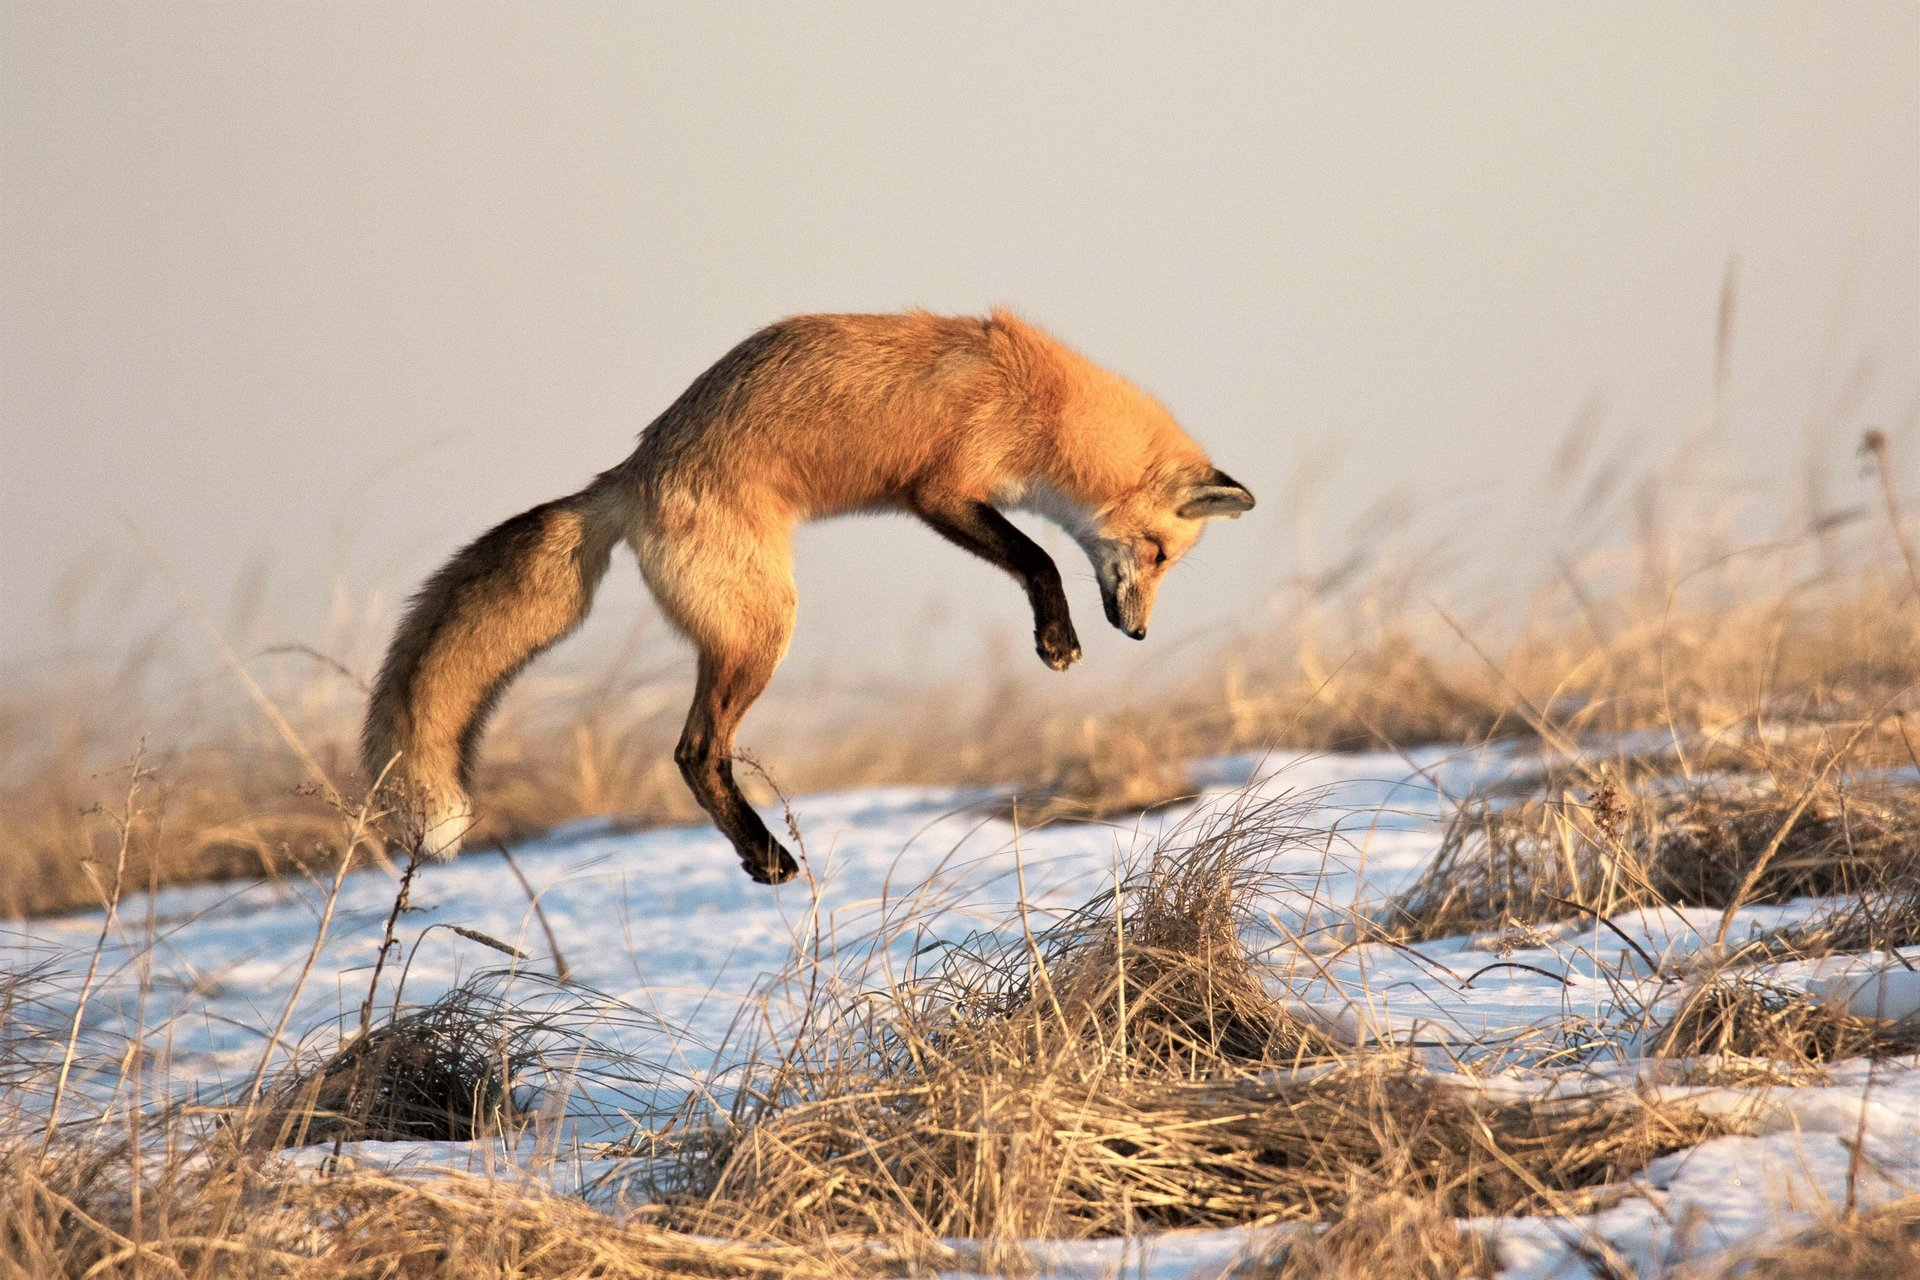
\includegraphics[width=1\textwidth]{pictures/hunter_lisek.jpg}
    \caption{Foxes are skilled hunters.}
    \label{fig:fox}
\end{figure}

If the probability of seeing a fox on a given day is \( p \), then the probability of seeing \( k \) foxes over \( n \) days follows a binomial distribution: 
\[P(n, k) = \binom{n}{k} p^k (1 - p)^{n -k}\]

Foxes are fascinating creatures known for their adaptability and cunning nature. Belonging to the Canidae family, they are found on every continent except Antarctica. The most common species, the red fox (\textit{Vulpes vulpes}), is particularly known for its striking reddish-orange fur, bushy tail, and sharp features. Foxes are primarily nocturnal, hunting at dusk and dawn, which allows them to avoid larger predators and take advantage of their keen sense of hearing and smell. Their diet is varied, consisting of small mammals, birds, insects, fruits, and even carrion, showcasing their opportunistic feeding behavior.
\par Socially, foxes are known for their \textbf{intelligence} and complex communication skills. They can emit a variety of sounds, from barks and screams to whines and howls, enabling them to communicate with other foxes and establish their territory. While often perceived as solitary animals, many species, including the red fox, form small family units to raise their young, called kits. The parental bond is strong, with both parents participating in the care and protection of the offspring. With their \underline{playful} demeanor and clever antics, foxes have become popular symbols in folklore and culture, often representing adaptability and cleverness in human storytelling.\paragraph{}

Foxes are great because:
\begin{itemize}
  \item[-] They're cute.
  \item[-] They're great hunters.
  \item[-] They're clever.
\end{itemize}

My tier-list of foxes:
\begin{enumerate}
  \item Red
  \item Arctic
  \item Fennec
\end{enumerate}
\paragraph{}
\textbf{The Comparison}\\
It is really hard to compare these great creatures, but take a look at the Table~\ref{tab:foxes}.
\begin{table}[htbp]
\caption{\textbf{Comparison}}
\label{tab:foxes}
\resizebox{\columnwidth}{!}{
\begin{tabular}{|l|l|l|l|}
\hline
\multicolumn{1}{|c|}{\textbf{Feature}} & \multicolumn{1}{c|}{\textbf{Red Fox}} & \multicolumn{1}{c|}{\textbf{Arctic Fox}} & \multicolumn{1}{c|}{\textbf{Fennec Fox}} \\ \hline
Habitat                                & Forests, urban areas                  & Tundra, Arctic regions                   & Deserts                                  \\ \hline
Diet                                   & Mammals, birds, fruits                & Rodents, carrion                         & Insects, small mammals                   \\ \hline
Lifespan                               & 3-5 years (wild)                      & 3-6 years (wild)                         & 10-14 years (captivity)                  \\ \hline
Body Size                              & 8-15 lbs (3.6-6.8 kg)                 & 6-21 lbs (2.7-9.5 kg)                    & 1.5-3.5 lbs (0.68-1.6 kg)                \\ \hline
Fur Color                              & Reddish-orange                        & White or gray                            & Creamy with large ears                   \\ \hline
Social Structure                       & Solitary or small groups              & Monogamous, family-oriented              & Solitary                                 \\ \hline
Adaptations                            & Highly adaptable                      & Thick fur, color change                  & Large ears, nocturnal                    \\ \hline
\end{tabular}
}
\end{table}